\documentclass[12pt, a4paper]{article}
\usepackage[ngerman]{babel}
\usepackage[utf8]{inputenc}
\usepackage[T1]{fontenc}
\usepackage{amsmath, amssymb}
\usepackage{geometry}
\usepackage{parskip}
\usepackage{booktabs}
\usepackage{array}
\usepackage{graphicx}
\usepackage{svg}
\usepackage{tikz}
\usepackage{siunitx}
\usepackage{fancyhdr}
\usetikzlibrary{trees, positioning}

\geometry{top=2.5cm, bottom=2.5cm, left=2.5cm, right=2.5cm}

\setlength{\parindent}{0pt}
\setlength{\parskip}{0.6em}

\newcommand{\punkte}[1]{\hfill \textit{(#1\,P)}}
\newcommand{\aufg}[1]{\medskip\noindent\textbf{A\,#1}\quad}

\pagestyle{fancy}
\fancyhf{}
\rhead{\thepage}
\lhead{}
\chead{}
\cfoot{Question Paper by Pravin}

\begin{document}

% ─── Header ────────────────────────────────────────────────────────────────────
\begin{center}
  {\LARGE\bfseries Test Paper for Mathematik}\\[0.4em]
{ 17. Mai 2026}\\[0.3em]
%  {\large\bfseries Mathematik II -- taschenrechnerfreier Teil}\\[0.2em]
%  {\large Aufgabengruppe A \quad Nachtermin (modifiziert)}
\end{center}

%\noindent Name: \underline{\hspace{6cm}} Vorname: \underline{\hspace{5cm}}

%\noindent Klasse: \underline{\hspace{2cm}} \quad Platznummer: \underline{\hspace{2cm}} \quad
%Punkte: \underline{\hspace{1.5cm}}\,/\,11{,}5

\bigskip

\bigskip

% ─── A 1 ───────────────────────────────────────────────────────────────────────
\aufg{1.0}
In einer Studie sollte für das Medikament~A (,,A``) und das Medikament~B (,,B``)
geprüft werden, ob sie wirksam (,,w``) oder nicht wirksam (,,nw``) sind.
Von den Personen, die an der Studie teilnahmen, bekamen \textbf{35\,\%} das
Medikament~A und die anderen das Medikament~B verabreicht.
Bei \textbf{38\,\%} der Personen, die das Medikament~B einnahmen, war dieses wirksam.
Betrachtet man die Personen, die das Medikament~A einnahmen, so war es bei
$p$\,\% $(p \in \mathbb{R}^+)$ wirksam.

\aufg{1.1}
Zeichnen Sie ein zugehöriges Baumdiagramm, in dem alle prozentualen Anteile
ersichtlich sind.
\punkte{2{,}5}

\vspace{2cm}

\aufg{1.2}
Von allen Personen, die an der Studie teilnahmen, wird eine Person zufällig
ausgewählt. Dabei erhält man mit einer Wahrscheinlichkeit von \textbf{21\,\%}
eine Person, die das Medikament~A einnahm und bei der dieses zugleich wirksam war.

Berechnen Sie den Wert von~$p$.
\punkte{2}

\vspace{4cm}

\bigskip
\hrule
\bigskip

% ─── A 2 ───────────────────────────────────────────────────────────────────────
\aufg{2.0}
Das folgende Baumdiagramm zeigt einen Zufallsversuch zum Ziehen von farbigen Kugeln.
In \textbf{Urne~1} befinden sich 16 Kugeln: 8 grüne (G), 6 schwarze (S) und 2 rote~(R).
Wird eine schwarze Kugel gezogen, so wird diese zurückgelegt und aus
\textbf{Urne~2} (7 Kugeln: 3 grüne, 4 rote) erneut gezogen (Wiederholung).
Die Wahrscheinlichkeiten der ersten Stufe betragen
$\tfrac{8}{16}$~(G), $\tfrac{6}{16}$~(S) und $\tfrac{2}{16}$~(R);
auf der zweiten Stufe (nach S) $\tfrac{3}{7}$~(G) und $\tfrac{4}{7}$~(R).

\aufg{2.1}
Beschreiben Sie einen Zufallsversuch, der zu einem analogen Baumdiagramm mit
\emph{vier} Ausgängen auf der ersten Stufe passt.
\punkte{2}

\vspace{3.5cm}

\begin{figure}[ht]
    \centering
    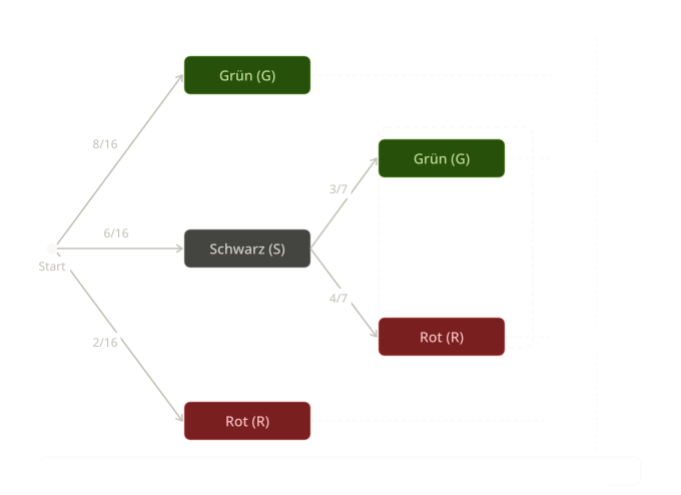
\includegraphics[width=0.5\textwidth]{baumdiagramm_A2_nachtermin.png}
\end{figure}

\aufg{2.2}
Geben Sie die Wahrscheinlichkeit dafür an, dass man beim Durchführen des
Zufallsversuchs aus A\,2.0 sofort eine grüne Kugel zieht \emph{oder} zuerst
eine schwarze Kugel und dann bei der Wiederholung eine grüne Kugel erhält.
\punkte{1}

\vspace{3cm}

\bigskip
\hrule
\bigskip

% ─── A 3 ───────────────────────────────────────────────────────────────────────

\aufg{3.0}
Die nebenstehende Zeichnung zeigt das Dreieck~$ABC$ mit
$|AB| = 9\,\text{cm}$ und $|AC| = 3\,\text{cm}$.
Die Eckpunkte $A$, $B$ und $C$ liegen auf dem Kreis~$k$ mit dem
Mittelpunkt~$M$ und dem Radius $r = 4{,}5\,\text{cm}$.

\aufg{3.1}
Begründen Sie, weshalb der Winkel $\angle ACB$ das Maß $90$\si{\degree} hat.
\punkte{1}
\begin{figure}[ht]
    \centering
    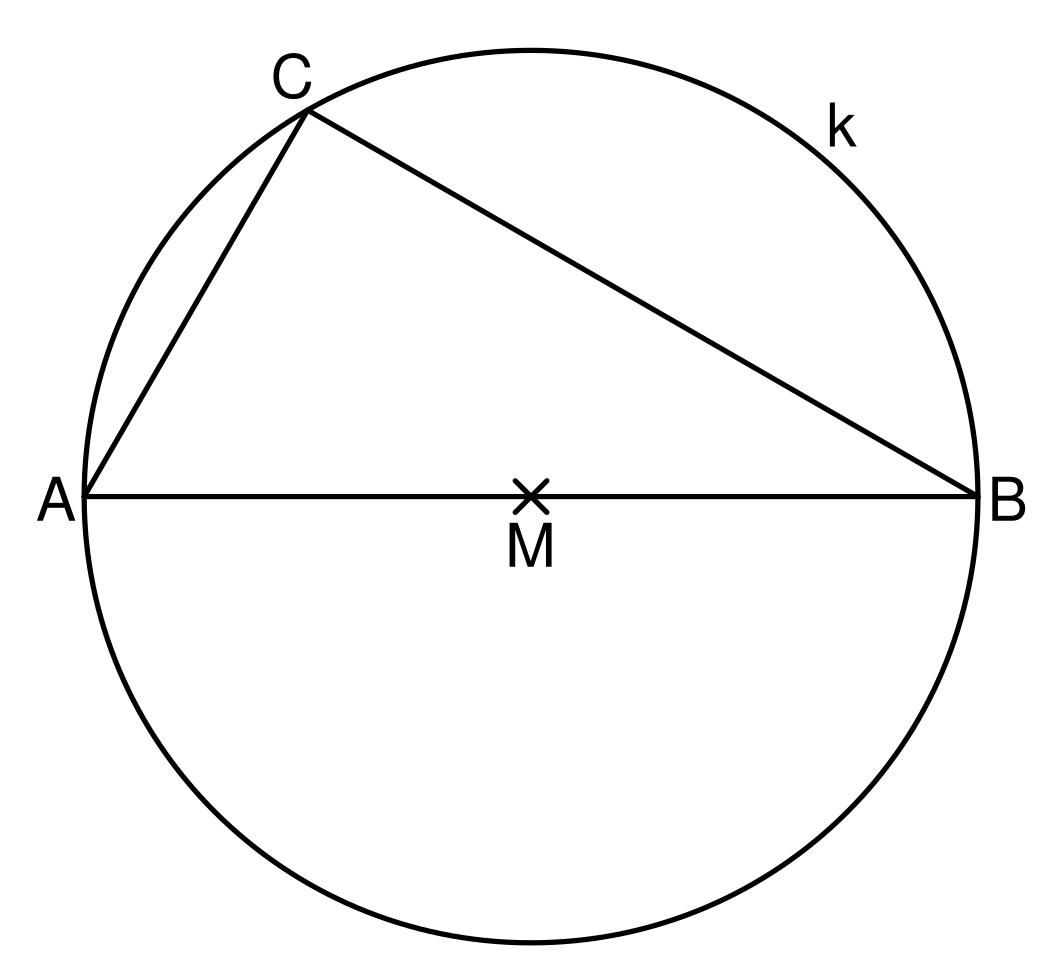
\includegraphics[width=0.3\textwidth]{Circle.png}
\end{figure}
\vspace{1cm}

\aufg{3.2}
Zeigen Sie, dass für das Maß des Winkels $\angle BAC$ gilt:
$\angle BAC \approx 70{,}5$\si{\degree}.
\punkte{1}

\vspace{0.5cm}

\aufg{3.3}
Bestätigen Sie rechnerisch, dass für den Flächeninhalt~$A$ des Dreiecks~$ABC$ gilt:
\[
  A = 9\sqrt{2}\;\text{cm}^2.
\]\punkte{2}


\end{document}